\subsection{End-to-End Results}
\label{sec:exp-e2e-results}

%1. overview & metric (3 sents)
Now we perform the cross-lingual table linking experiment and compare with
previous table linking and text linking systems.
%Recap that not all mentions in our dataset have a gold English entity.
%we only attempt to link those mentions with English labels (see Definition \ref{def:mention}).
%For mentions not to be linked,  are still helpful for the mention is still helpful, since it
%and exclude mentions  without a proper Chinese concept,
%or failed to transfrom into the equaivalent English concept.
To be consistent with state-of-the-art systems, we report Micro Accuracy
and Macro Accuracy as the evaluation metrics.
%Micro Accuracy, used in $TabEL_B$~\cite{bhagavatula2015tabel} and
%$TabEL_W$~\cite{wu2016entity}, is the fraction of cells
Micro Accuracy is the percentage of correct linked cells over the whole dataset,
%where the predicted entity exactly matches the labeled English concept.
whiles Macro Accuracy, defined as average correct ratio over different tables,
%defined as the fraction of correctly linked cells averaged over all tables,
avoids the bias towards the table with more cells.

%2. show result, overall statement (3 sents)

%In order to keep a fair comparison,
Due to both $TabEL_B$ and $TabEL_W$ taking only one English mention per cell as the input,
we select Baidu as the best translation tool and apply this setting to all approaches.
In addition, we evaluate our approach under the full translating strategy,
using either pre-train or without pre-train.
For all the variations of our approach,
we set $N_{cand}=30$, $N_{tab}=49$, $d_{cell}=d_{cont}=100$, $d_{out}=200$, $\eta=0.0002$ and $p=0.9$ under RankNet optimizer,
as reaching the highest Micro Accuracy in the validation set.
For other approaches, we use different $N_{cand}$, tuning separately.

We report the experimental results in \tabref{tab:main-result}.
For the 4 experiments using Baidu translation only, 
Our model outperforms the other baseline models, improving the result by up to 12.1\%.
Our full model even improves the Micro Accuracy by an absolute gain of 0.053,
showing the importance of combining multiple translating tools.
Besides, the pre-train step also raises the Micro Accuracy by 0.023.
%3. compared with TabEL, ()
Both $TabEL_B$ and $TabEL_W$ suffer from the error propagation problem,% in the translating step,
because only the top translation is considered,
%as the mono-lingual approaches take translated mentions
%as direct input, a poor translating quality harms the final result.
whereas our approach generates candidate entities from multiple translated mentions,
%takes Chinese mention as the input, such end-to-end approach
which alleviates the error brought by translation.
%4. compared with Wu
%Compare our approach with $TabEL_{Ch}$, it's no suprise to observe that,
%the mono-lingual table linker keeps competitive under the perfect translation
%of Wiki concepts from Chinese to English, but the gap between theirs and our approach
%(xx.x versus xx.x) is relatively small.
%\KQ{So shall we add another experiment? Use Wiki-inter-link to generate candidates ?}
%5. compare with text EL (Wiki inter-link, ours)
%6. Summary

%We show the experimental results in \tabref{tab:main-result}.
%Our model outperforms previous work and improves the acurrency by a relative gain of xx\%.
%For TabEL, the linking accuracy is limited by the quality of translated English table.
%By manually inspecting the translated English mentions, the translation accuracy is around xx\%,
%which is close to our quality of English candidate generation in \secref{sec:cand-gen-eval}.


\begin{table}[ht]
\small
\centering
\caption{Accuracies on cross-lingual table linking task.
All baselines take Baidu as the only translating tool.}
\label{tab:main-result}
\begin{tabular} {c|c|cc}
    \hline
    Approach          & Micro Acc.   & Macro Acc.    \\
    \hline
    $TabEL_B$         &  0.512       & 0.507         \\
    $TabEL_W$         &  0.514       & 0.519         \\     %N_{cand} = 10
    $TextEL$          &  0.472       & 0.458         \\
    Ours (Baidu Only) &  0.576       & 0.573         \\
    \hline
    Ours (Full, - pre-train) &  0.606    &  0.591        \\ 
    Ours (Full, + pre-train)  &  \textbf{0.629}       & \textbf{0.614}         \\
    \hline
\end{tabular}
\end{table}

We further investigate how the candidate size of a mention effects the table linking result.
%The intuition is that,
When $N_{cand}$ goes larger, the theoretical upper bound of the final result increases,
%however, with more negative candidates been introduced,
but it's more difficult for the system to reach the upper bound.
%Therefore, we perform the experiment under different $N_{cand}$ and investigate how
%does each model handle this tradeoff.
For analyzing such tradeoff,
\figref{fig:main-result} shows the Micro Accuracy trend of each approach,
and we display upper bound (Hits@$n$) in the figure.
%From the results, we observe that the Micro Accuracy increases when $N_{cand}$ is small,
%and then decreases when $N_{cand}$ goes larger.
Our approach is more adaptive to different size of candidates,
and can produce promising end-to-end results.
$TabEL_B$ also keeps a stable performance with a subtle decreasing, 
while $TextEL$ drops dramatically, even if the candidate size is smaller than 10.
The main reason is that BLDA model is unsupervised, which doesn't observe any explicit
(mention, entity) pair for learning.
%Two main reasons are:
%1) the BLDA model is unsupervised, though equivalent articles between
%Chinese and English Wikipedia pair together as the input documents, the model doesn't observe
%any explicit (mention, entity) pair for learning,
%2) the similarity between the mention and the entity is only determined by their topic
%distributions, without features derived from entity names, or from coherence information.
%These reasons make $TextEL$ much more sensitive to noisy candidates.

%with less error propagation during the translation step,


\begin{figure}[th]
\centering
%\epsfig{file=fb-schema-4.eps, width=0.95\columnwidth}
\scalebox{0.25}{\includegraphics[angle=0]{figures/main-result-crop.eps}}
\caption{Results of Micro Accuracy varied from different size of candidates,
using Baidu translation only.}
\label{fig:main-result}
\end{figure}




